While in the previous chapter we detailed the experimental setup and infrastructure, in this one we will show all results about the performance from distributed training and from the learned kick motions.

\section{Distributed Training}

The first results we show here are regarding of data parallelism by the adoption of distributed training. In RL setup, we used a master-worker model (as described in Subsection \ref{sec:distributedtraining}) with \textbf{108 agents} collecting data in parallel.

We used Intel AI DevCloud \cite{inteldevcloud}. It is a cluster of Intel Xeon Scalable Processors that assists with machine learning and deep learning research, with several optimizations for this domain. We had available 10 computation nodes, each of them with 24 cores for processing. Therefore, we trained using 9 nodes for workers (each of them with 12 agents) and one node for master computation. All the scripts used for training configuration are available in the github repository\footnote{\label{scripts} https://github.com/luckeciano/deep-rl-humanoid-kick} of this work. 

In Figure \ref{fig:speeduptest}, we see how the data collection had improved by using distributed training in AI DevCloud. In this graph, we have the number of samples collected by learning update in a training using the distributed configuration and other in a local training with a single agent. 

\begin{figure}[!htbp]
	\centering
	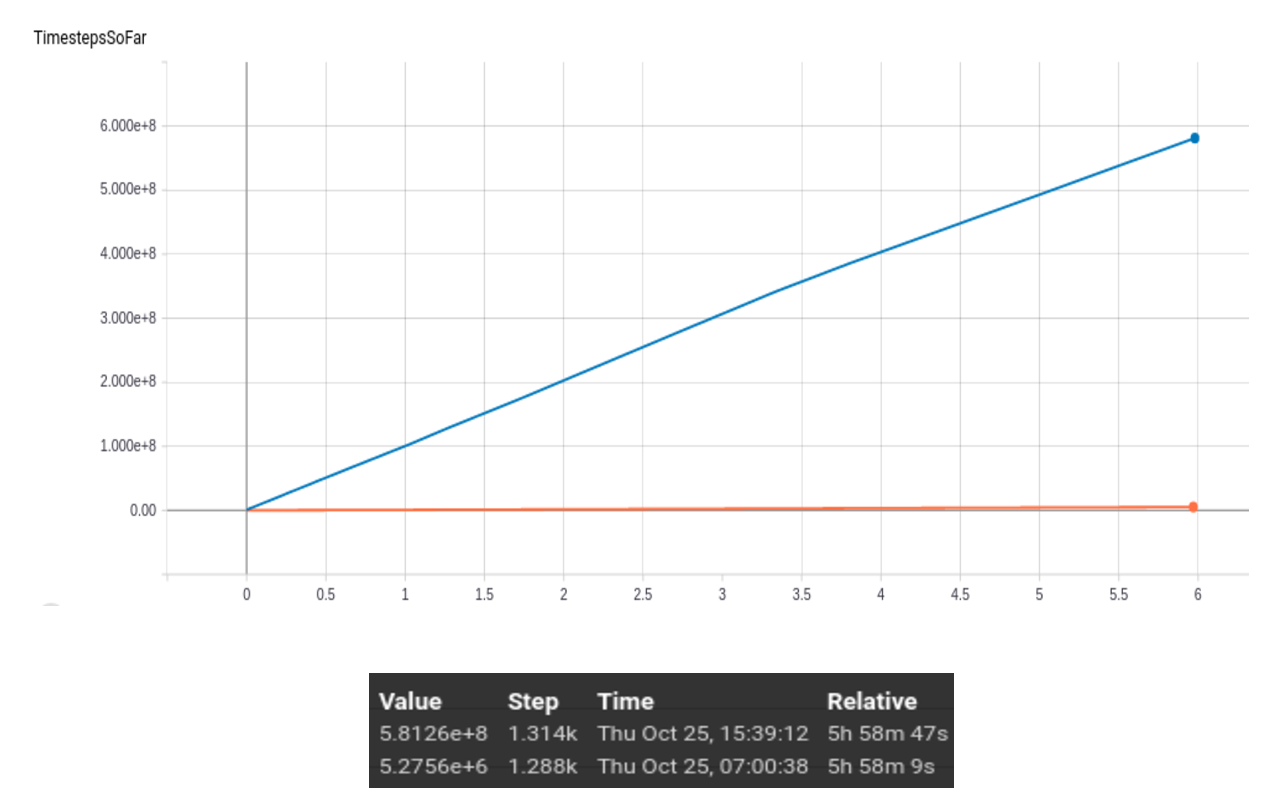
\includegraphics[width=1\textwidth]{Cap6/speeduptest}
	\caption{Speedup Test}
	\label{fig:speeduptest}
\end{figure}

If we consider the same instant at each experimentation (i.e, after the same period of time), we can quantify the speedup:

\begin{equation}
	SpeedUp \approx \frac{5.81 * 10^{8}}{5.27 * 10^{6}} \approx \textbf{110}.
\end{equation}

In this comparison, we have a speedup of 110. It is interesting the fact that the speedup is greater than the number of agents. It worth mentioning that this number can vary depending on the training itself, because the computation will change over time. For example, if during training the episode length tends to grow, the time simulating agents have the same behavior. Therefore, the reason of this speedup is that the training may have been conducted for a computation that collects more data rather than computing more network updates


In Figure \ref{fig:absdatacollection}, we consider the best scenario for data collection from those experiments. In the graph, there is the number of samples collect by the time.
In this example, we have collected approximately \textbf{740 millions of samples} in eight hours. It means \textbf{92.5 millions of samples by hour}. Each of them means a cycle of 20 milliseconds in the simulation server. Therefore, we collected approximately \textbf{21.4 days of real time training in each hour of simulation}. The training from Figure \ref{fig:absdatacollection} collected approximately \textbf{171 days of uninterrupted training} -- almost half year.

\begin{figure}[!htbp]
	\centering
	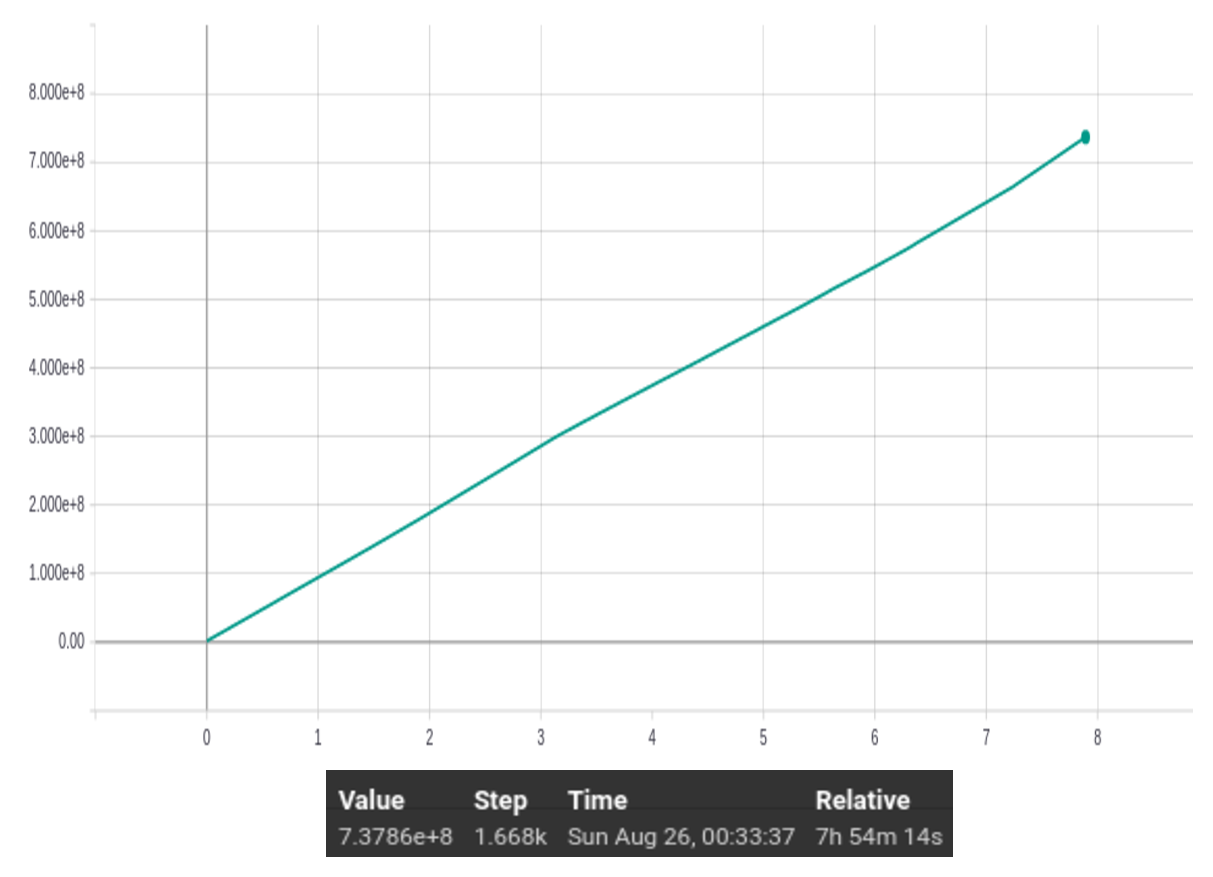
\includegraphics[width=1\textwidth]{Cap6/absolutedatacollection}
	\caption{Data collection in best scenario}
	\label{fig:absdatacollection}
\end{figure}



\section{Pure Reinforcement Learning Methods Results}

In this section, we show the results regarding of RL experiments. We tested several scenarios using the experimentation setup described in Section \ref{sec:experimentation_setup}. All the hyperparameters from each experiment can be found in the Appendix \ref{ap:hyperparameters}.

\subsection{RNR}\label{sec:rnr}

The first model we experimented is the RNR. In this, we started from randomly distributed weights in a neural network and, by using RL, we achieved a motion that not follows a well-defined human kick behavior, but is able to inject some velocity to the ball. Figure \ref{fig:rnrreward} shows how the reward improves over the learning process.

\begin{figure}[!htbp]
	\centering
	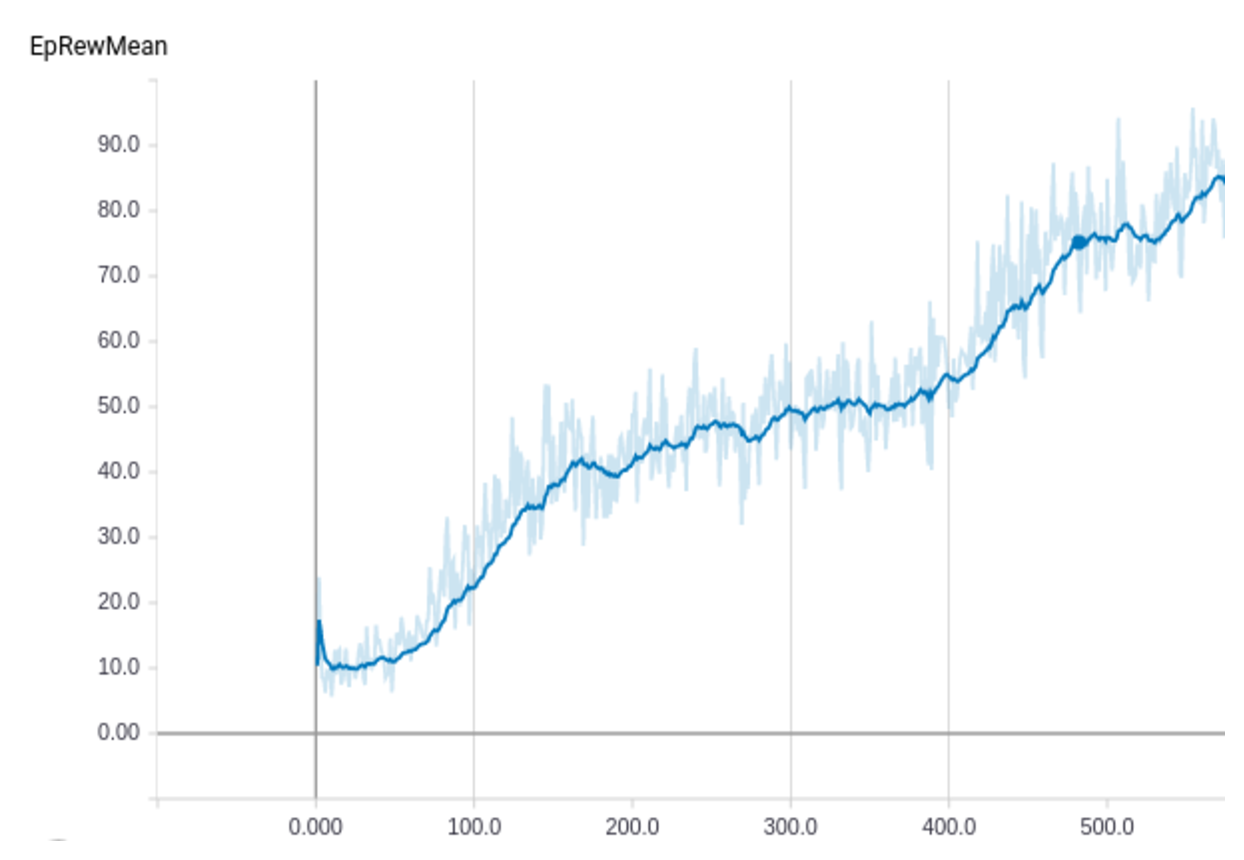
\includegraphics[width=0.8\textwidth]{Cap6/rnrreward.eps}
	\caption{RNR Reward Curve by learning update}
	\label{fig:rnrreward}
\end{figure}

Other experimentation sessions shown us that RNR tends to converge to the maximum value presented in Figure \ref{fig:rnrreward}.

We also encountered a problem during the optimization process: Simspark simulation tends to drastically drop the reward to zero after approximately 4 or 5 hours of training in certain experiments. We did not find a reason but when we restart training from the previous session, the problem just disappear. We opted to not show this issue in results to not compromise the focus of the research.

Figure \ref{fig:rnr_kick_sequence} shows RNR resultant motion. It is possible to see that the behavior is different from the human kick pattern. Basically, the robot jumps and push its right leg in ball direction. This kick runs between two to four meters straight. A video showing the animation may be seen in the repository.

\begin{figure}[!htbp]
	\centering
	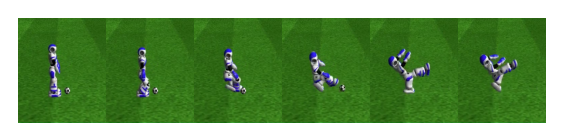
\includegraphics[width=1.0\textwidth]{Cap6/rnr_kick_sequence.eps}
	\caption{RNR kick motion sequence.}
	\label{fig:rnr_kick_sequence}
\end{figure}

\subsection{RRR}\label{sec:rrr}

In the context of optimization it is difficult to the agent explore the whole action space and mimics a human behavior of kicking. To address this challenge, we used the reference motion also used in supervised learning section.

When we train just using this reward -- without any reward to kick the ball itself -- the robot achieves a interesting behavior: it remains stopped, even growing the reward, as in Figure \ref{fig:rrrreward}.

\begin{figure}[!htbp]
	\centering
	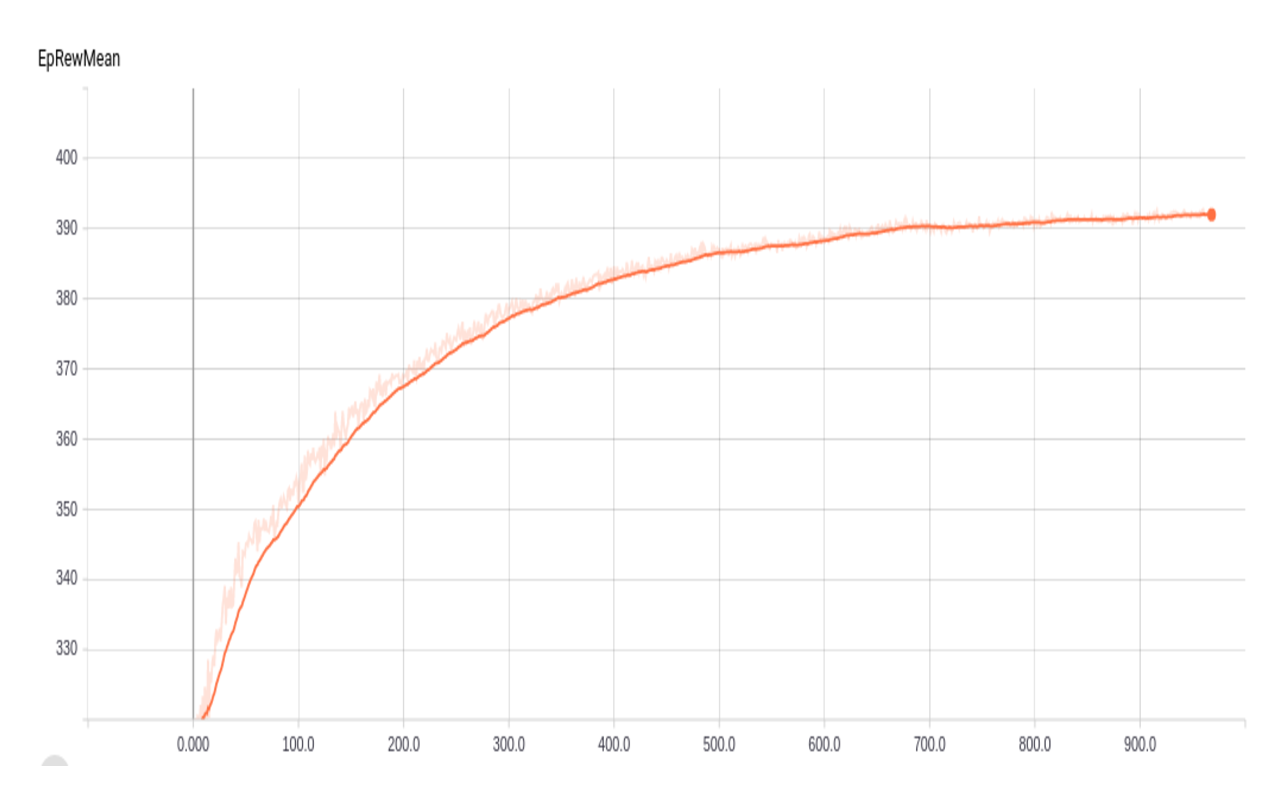
\includegraphics[width=0.8\textwidth]{Cap6/rrrreward.eps}
	\caption{RRR Reward Curve by learning update}
	\label{fig:rrrreward}
\end{figure}

Actually, we hypothesize that this behavior happens because it is better for the agent remains in the same position with a stabilized error than tries to reduce this error and possibly fall -- which will result in a much worse reward if compared to just stand still.

\subsection{RNR+RRR}

A possible solution for RNR and RRR models is to join both in one single solution. It will avoid weird motion from RNR configuration by using a reference and will also reinforce positively the task of moving the ball.

Indeed, the resultant motion captures these two ideas and generates a new behavior, which looks more like a human pattern for kicking. We present the training curve for the best experiment in Figure \ref{fig:rnrrrrrewardcurve} and the motion sequence in Figure \ref{fig:rnrrrrreward}.

\begin{figure}[!htbp]
	\centering
	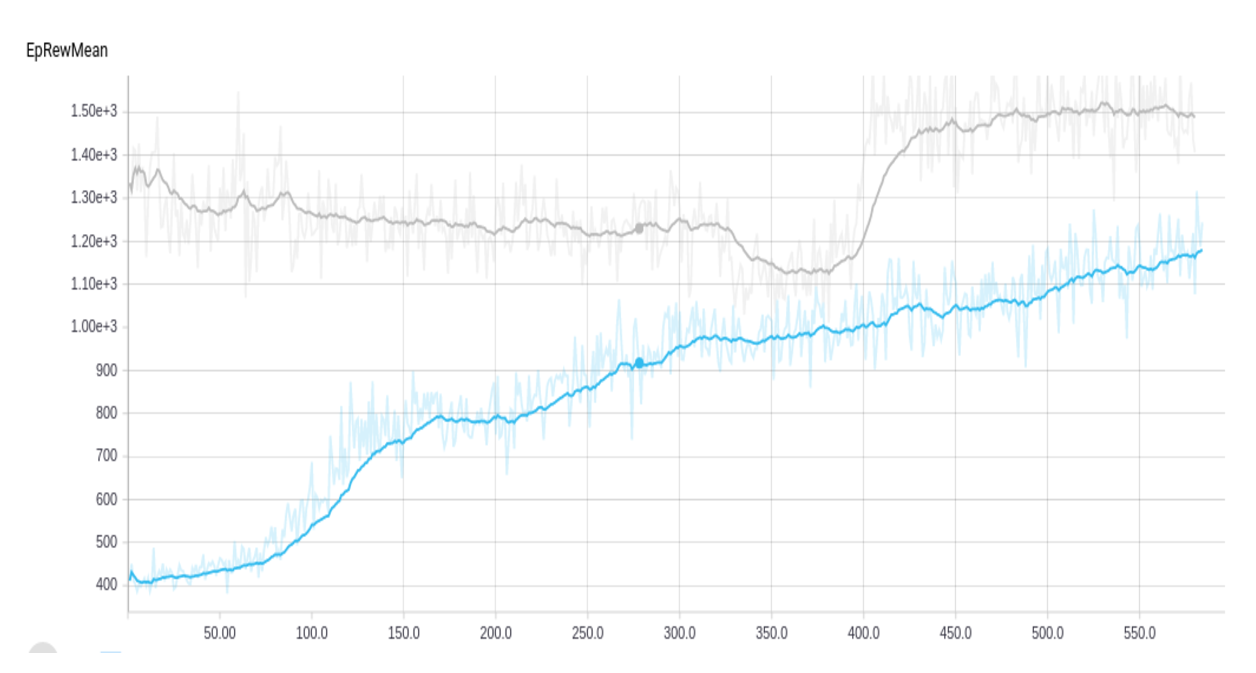
\includegraphics[width=0.8\textwidth]{Cap6/rnrrrrrewardcurve.eps}
	\caption{RNR+RRR Reward Curves by learning update. We trained in two sessions. The blue curve shows the first session and the gray one the second session.}
	\label{fig:rnrrrrrewardcurve}
\end{figure}

One fact that is interesting to mention: in RNR motion (without reference), the agent learns to kick with the right leg. In this model, on the other side, the agent learns to kick with the left leg, as in the reference motion.

\begin{figure}[!htbp]
	\centering
	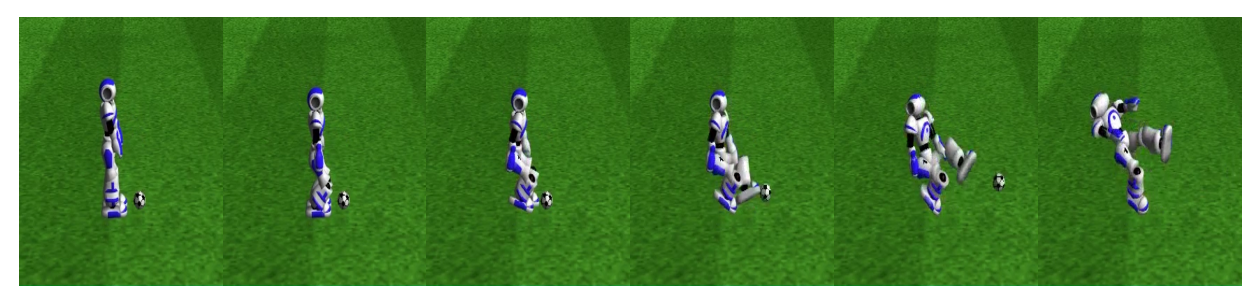
\includegraphics[width=1.0\textwidth]{Cap6/rnrrrrreward.eps}
	\caption{RNR+RRR Motion Sequence. In this model, the agent learns to kick with the left leg, as in the reference.}
	\label{fig:rnrrrrreward}
\end{figure}


The big challenge of this model is to tune the weight parameter for each reward. If we use much greater reward for moving the ball, the model collapses to the RNR configuration. On the other side, if the reference reward is much greater, it collapses to the RRR. It is a trade-off and is very difficult to tune this kind of parameter manually. Figure \ref{fig:rnrrrrtradeoff} shows a collapse case.


\begin{figure}[!htbp]
	\centering
	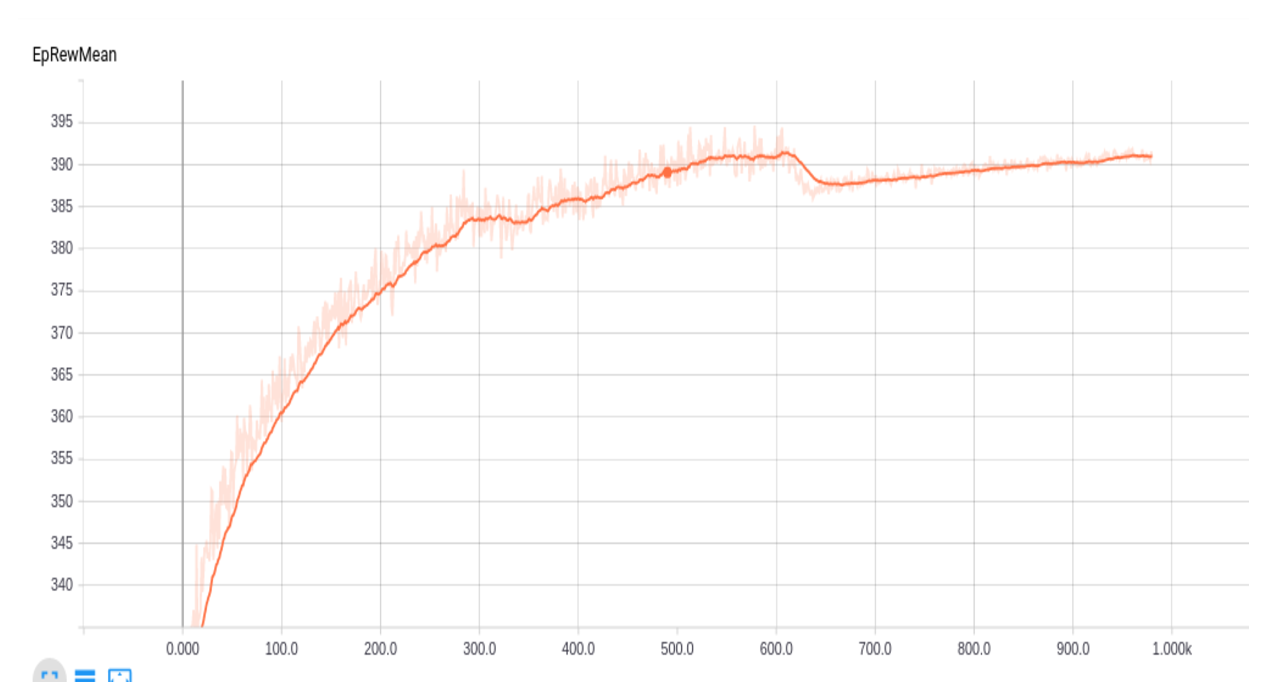
\includegraphics[width=1.0\textwidth]{Cap6/rnrrrrtradeoff.eps}
	\caption{Tradeoff between RNR and RRR models: when parameter weight for RRR is much greater, it collapses to RRR model.}
	\label{fig:rnrrrrtradeoff}
\end{figure}

\subsection{RNR+RRR+RISD}\label{sec:rnrrrrrisd}

Even joining RNR and RRR, the agent is not able to learn the main patterns from the kick motion. It is difficult to learn, for example, that the leg should go back before making the move.

The main reason for this challenge -- even when we pass the reference motion -- is because the training is intrinsically sequential. It means that the later stages is achieve only if all previous states are satisfied. Otherwise, The agent will probably fall and not complete the episode.

Using the RISD model, we can train the whole motion ``in parallel". We show the training curve from RNR+RRR+RISD model in Figure \ref{fig:rnrrrrrisdcurve}. 

\begin{figure}[!htbp]
	\centering
	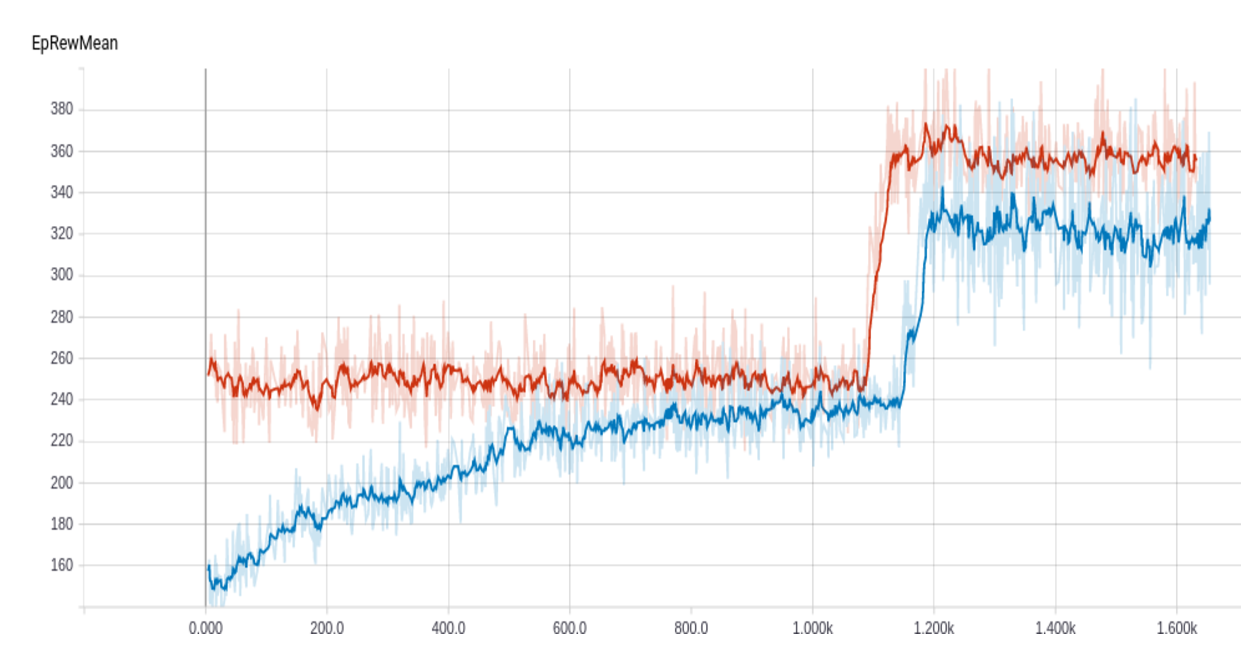
\includegraphics[width=1.0\textwidth]{Cap6/rnrrrrrisdcurve.eps}
	\caption{RNR+RRR+RISD learning curve in two sessions of training. The blue curve was the first session and the red one was the second.}
	\label{fig:rnrrrrrisdcurve}
\end{figure}


During the first session of training, the first thousand updates were related to reduce the error from the reference motion. It is similar to the curve from RRR model. After this, the model grows drastically until a new baseline. It corresponds to the moment where the agent, by exploration, achieves the situation of completing the whole motion.

The second session starts from the first one. However, the first part of the training is comparable to the result before the drastic grow from first session. Then, by exploration, the reward drastically grows again, but for a second baseline, higher.

Comparing the result from both training, the second baselines is able to kick the ball following the reference motion; the first is not.

Figure \ref{fig:risdmotionsequence} shows the motion sequence from RNR+RRR+RISD model. It is a complex and detailed motion. Although it is able to kick the ball, it is a rare situation and hardly ever achieves 3 meters. The big problem of this motion is the beginning: the agent fails in maintain a support foot. Nevertheless, the pure reinforcement method was able to mimic the human behavior of kicking.

\begin{figure}[!htbp]
	\centering
	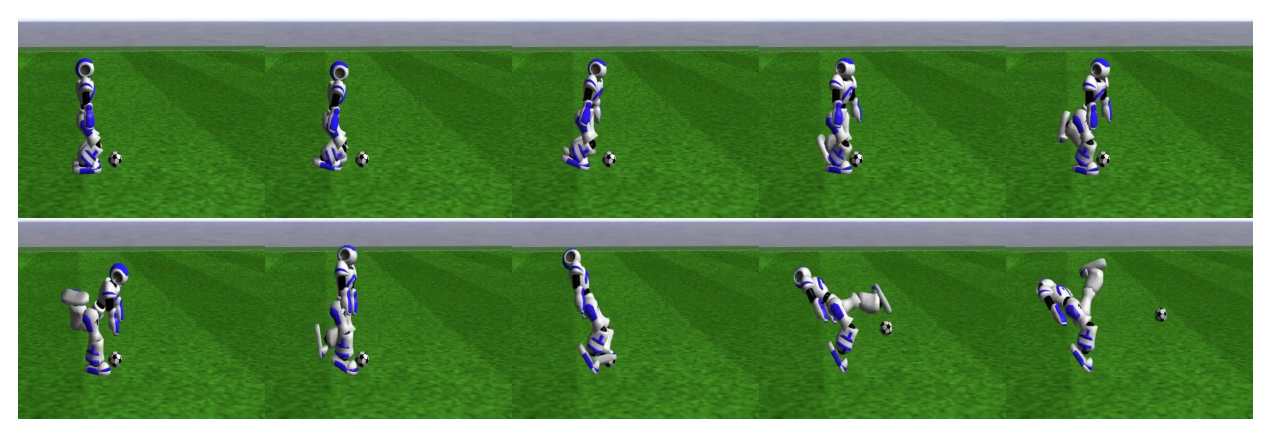
\includegraphics[width=1.0\textwidth]{Cap6/risdmotionsequence.eps}
	\caption{RNR+RRR+RISD motion sequence.}
	\label{fig:risdmotionsequence}
\end{figure}


%\subsection{RNR+RRR+RISD+RET}

%This final experiment using pure RL techniques tries to improve last model by using Early Termination. As we saw in Figure \ref{fig:rnrrrrrisdcurve}, the training curve is unstable and depends by the right situation of exploration to achieve a reasonable baseline. Considering the model, there is cases where the agent falls but we keep collecting data until the end of a fixed number of samples. Therefore, we collect a lot of wrong data that can harm learning.

%Figure \ref{fig:finalpurereward} shows RNR+RRR+RISD+RET model. 

%\begin{figure}[!htbp]
%	\centering
%	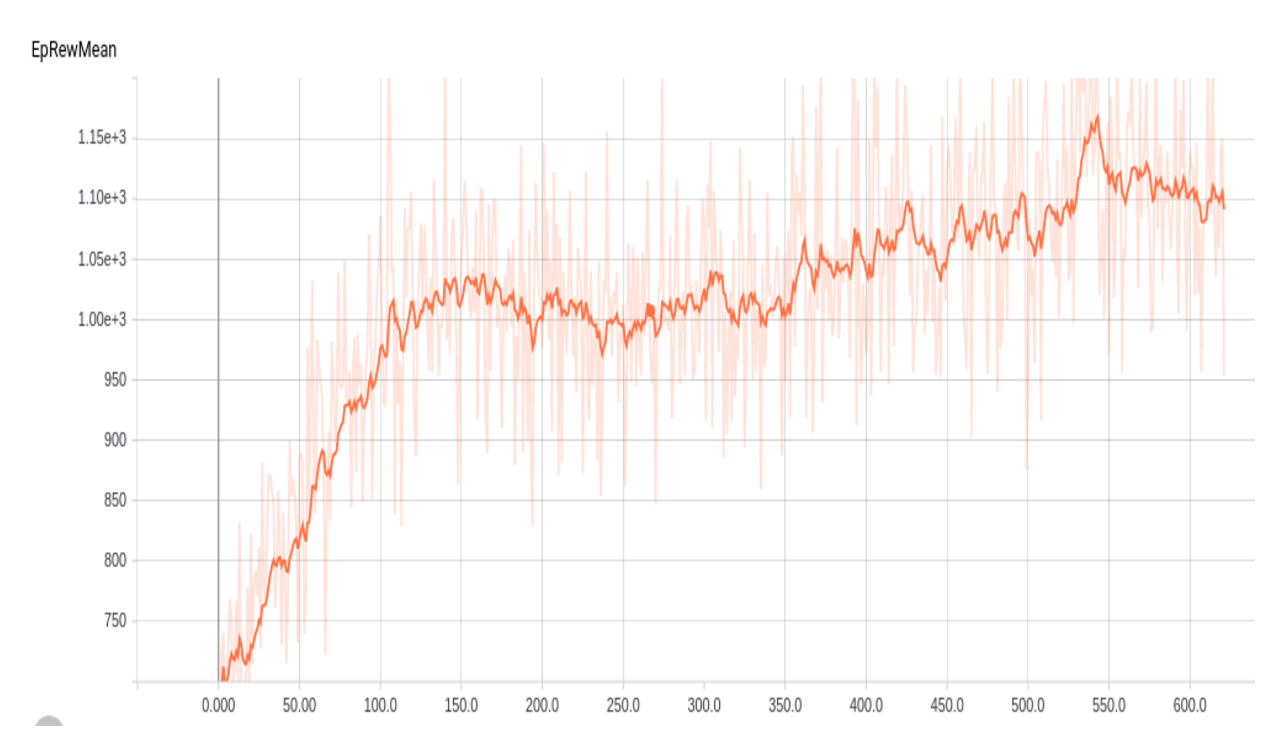
\includegraphics[width=1.0\textwidth]{Cap6/finalpurereward}
%	\caption{RNR+RRR+RISD+RET reward curve.}
%	\label{fig:finalpurereward}
%\end{figure}

\subsection{Reinforcement ``Supervised"}\label{sec:suprl}

As a mid-term between pure RL techniques and HLM model, we propose a reinforcement ``supervised" learning model, where we use only the PPO algorithm but as initial stage we use the reference motions as a dataset $(x, y)$ where $x \in \mathcal{S}$ and $y \in \mathcal{A}$ and the reward is the opposite of mean absolute error:
\begin{equation}
R(x) = - \lvert \hat y(x) - y(x) \rvert.
\end{equation}

 In this way, we reduce RRR model to a ``supervised" problem without the simulation. This model breaks the sequentially of data, since the states are used in the training in isolation and not as a reflection of the horizon prior to this, satisfying Markov property.

Figure \ref{fig:rlsupcurves} shows the first of six training sessions for a reinforcement supervised configuration, using mean absolute error as penalization. It shows to be a bit difficult to converge -- the optimization is very sensible to learning rate value. In each training session, we needed to tune this hyperparameter again.

\begin{figure}[H]
	\centering
	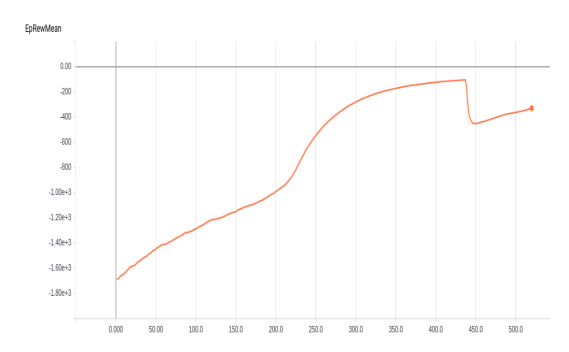
\includegraphics[width=1.0\textwidth]{Cap6/rlsuprewardcurves.eps}
	\caption{First session of training for reinforcement supervised model.}
	\label{fig:rlsupcurves}
\end{figure}

Although the learned motion mimics the reference, it accumulates error at the end of the motion and ends up kicking the floor, as shown in Figure \ref{fig:rlsupmotionsequence}. For this reason, it could not be used as seed for new kick policies.

\begin{figure}[H]
	\centering
	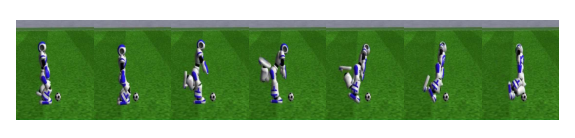
\includegraphics[width=1.0\textwidth]{Cap6/rlsupmotionsequence.eps}
	\caption{Motion sequence from reinforcement supervised learning agent.}
	\label{fig:rlsupmotionsequence}
\end{figure}

\subsection{Other ideas for pure RL techniques}

There are other possible ideas to explore in order to obtain a reasonable copy from the reference motion to use as seed for optimization. Analyzing the experiments described in this section until now, we found out we have two main problems:

\begin{itemize}
	\item The agent is not able to learn a stable support foot, compromising the later stages of kicking; and
	\item The kicking foot sometimes hits the ground and not the ball.
\end{itemize}

To address these problems, we need domain-specific rewards to ensure stability, such as:

\begin{itemize}
	\item Consider the center of pressure that the support foot does on the ground; the more centralized is this pressure, the more stable the kick should become \cite{phdmanga};
	\item Consider the curve that kicking foot and leg do in relation to torso during reference motion; and
	\item Consider torso coordinates from reference motion during training \cite{peng2018}.
\end{itemize}

We preferred not to explore these ideas because as we will see in next section, hybrid learning models worked much better and easier. Furthermore, in this work, we aim to explore non domain-specific techniques that could be generalized for other kinds of motions.

It is worth mentioning that the techniques explored until now worked well,even without a seed motion for bootstrapping the learning. Fitting this specific reference motion is really difficult because it has high performance and, therefore, the robot operates close to the limit of stability. However, in other motions, they are good tooling for mimicking.

\section{Hybrid Learning Models}
In this section, we will explore an alternative for pure RL methods -- what we called Hybrid Learning Models. In this configuration, there is a pre-training step where we used supervised learning algorithms to fit the reference motion before using the PPO algorithm.

\subsection{Supervised Learning Results}\label{sec:slresults}
The first results from Hybrid Learning Models are related to the supervised learning step where we copy the motion from keyframe representation to neural network one. We evaluate this model not just in kick motion, but also learning the walking engine and other keyframe motions, such as the get up motion.

\subsubsection{Training Results}

\begin{figure}[H]
	\centering
	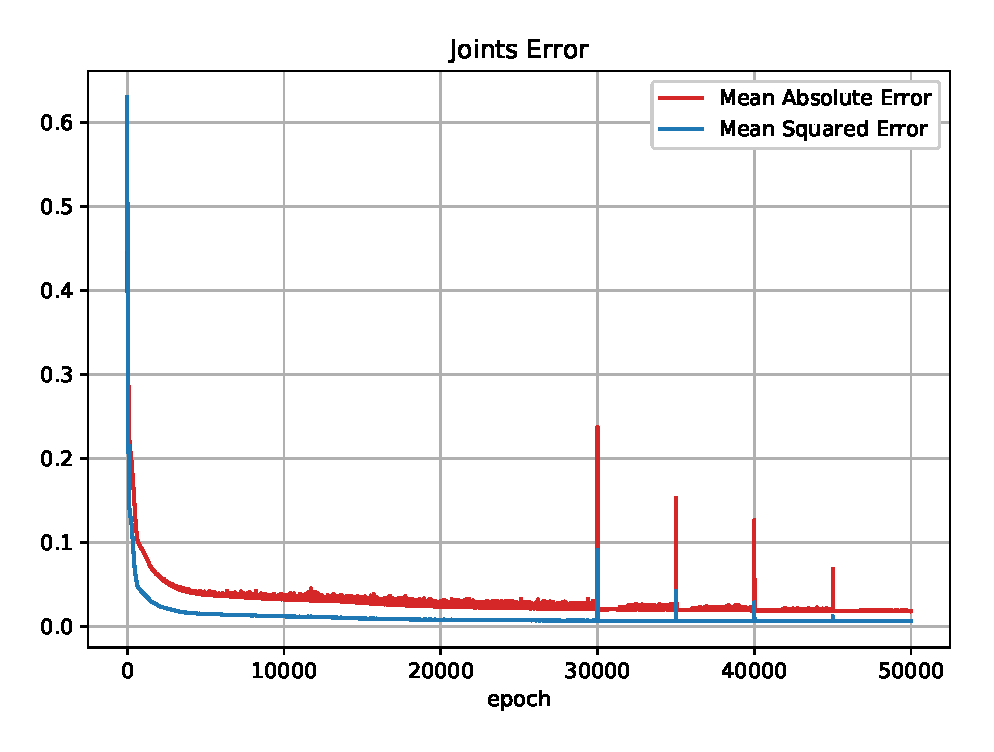
\includegraphics[width=1\textwidth]{Cap6/errors}
	\caption{Plots of mean squared error and mean absolute error, during training.}
	\label{fig:errors}
\end{figure}

The initial results came from the training procedure, outside the simulation environment. Figure \ref{fig:errors} presents training curves for the kicking keyframe dataset. In this case, plots show the mean squared error and the mean absolute error metrics. In both metrics, the value drastically decreases in the first epochs. This same behavior was present in other training procedures as well. However, only after thousands of epochs, the network has achieved a low error that successfully reproduced the motion, which has shown how sensible to small joint errors keyframes were, given that they are open-loop motions. The peaks, during the training has happened at the learning rate transition instants, but they did not hurt the training procedure itself.

\subsubsection{The Learned Kick Motion}

The final mean absolute error was \textbf{0.018} radians and the motion was visually indistinguishable from the original one, as can be seen in Figure \ref{fig:motions}. In this figure, snapshots from both motions were taken. Figure \ref{fig:kick_joints_curves} shows several plots of joint angles, by comparing the original and learned kick motions. As we may see, the learned motion has fitted the movement with minor errors\footnote{\label{footnote_walk} Kick results video: https://youtu.be/UAbqQLUnvDo}.

\begin{figure}[H]
	\centering
	\includegraphics[angle=90,width=1\textwidth]{Cap6/motions}
	\caption{The kick motion. The first row of figures shows the original kick motion. The second row shows the learned kick motion. Both motions are visually indistinguishable.}
	\label{fig:motions}
\end{figure} 

In order to evaluate the learned kick motion in the RoboCup Soccer 3D domain, we created a statistical test. Inside the test scenario, the ball was initially placed in the center of the field with an agent near to it. The only action of the agent was to kick the ball in the goal direction. After the kick, the agent run until reaching the ball and kicked it again, repeating this process till scoring a goal. When the goal has occurred, this same scenario was repeated. The whole test was conducted, during thirty minutes in clock time and the following data was collected: total number of kicks, number of successful kicks, mean distance that the ball has traveled, and the standard deviation of this measure. The results from the original and learned kicks are shown in Table \ref{tab_kicks_statistics}.


\begin{figure*}[!htbp]
	\centering
	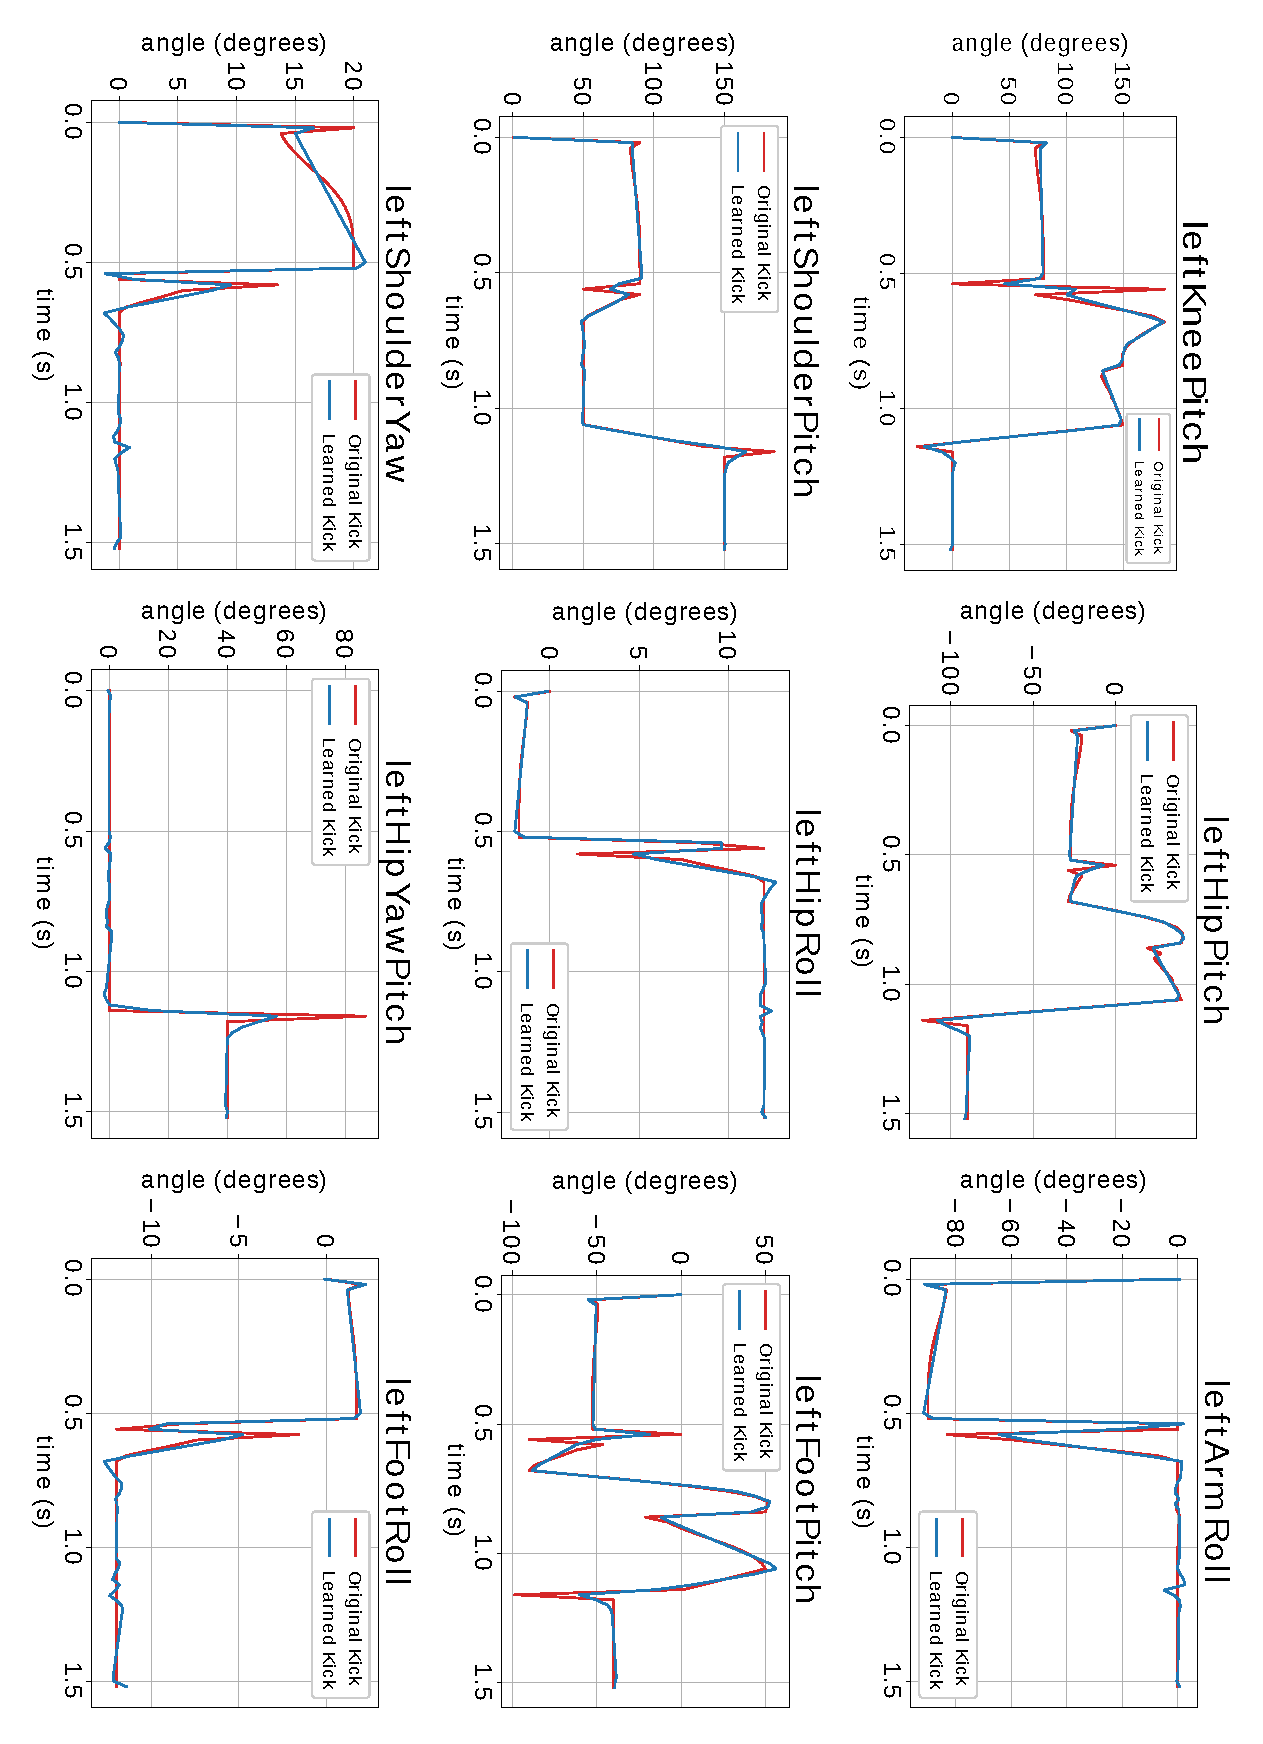
\includegraphics[angle=90,width=1\textwidth]{Cap6/kick_joints_curve}
	\caption{Joint values for comparing original and learned kicks. The neural network was able to fit the joint trajectories with small errors.}
	\label{fig:kick_joints_curves}
\end{figure*}


\begin{table}[htbp]
	\caption{The Kick Comparison}
	\begin{center} 
		\begin{tabular}{|c|c|c|c|}
			\hline
			\textbf{Kick}&\multicolumn{3}{|c|}{\textbf{Statistics}} \\
			\cline{2-4} 
			\textbf{Type} & \textbf{\textit{Accuracy (\%)}}& \multicolumn{2}{|c|}{\textbf{Distance (\(m\))}} \\ 
			\cline {3-4}
			& & \textbf{\textit{Mean}}& \textbf{\textit{Std}} \\
			\hline
			Original Kick & 64.5 & 8.92 & 3.82  \\
			\hline
			Neural Kick & 52.6 & 7.16 & 4.06 \\
			\hline
		\end{tabular}
		\label{tab_kicks_statistics}
	\end{center}
\end{table}

Although both kicks had similar results, the original kick was slightly better in this scenario. By confronting Figure \ref{fig:kick_joints_curves}, we can conclude that even with an almost equal representation, the kick lost part of its efficiency and this fact has shown how sensible were movements based on keyframe data.

\subsubsection{The Learned Walk Motion}
By using the modified server described in Subsection. \ref{AA}, a dataset with samples of the UT Austin Villa's walking motion \cite{macalpine2013} was acquired. This team is the current champion of the RoboCup Soccer 3D competition \cite{macalpine2017}.

The objective was to mimic the walk motion as a keyframe and use this motion in our agent. The previously described framework for learning our own kick motion was used in this training, by including the neural network architecture and its hyperparameters.

The results from this training are shown in Figure \ref{fig:walk_joints_curves}. Similarly to Figure \ref{fig:kick_joints_curves}, it shows the joint angles throughout the walking motion period for the original and learned walk. Additionally, it shows the real joints values from the movement in the server. These joints were chosen because they were the most dynamic in the walk motion and, therefore, the hardest to learn.

\begin{figure*}[!htbp]
	\centering
	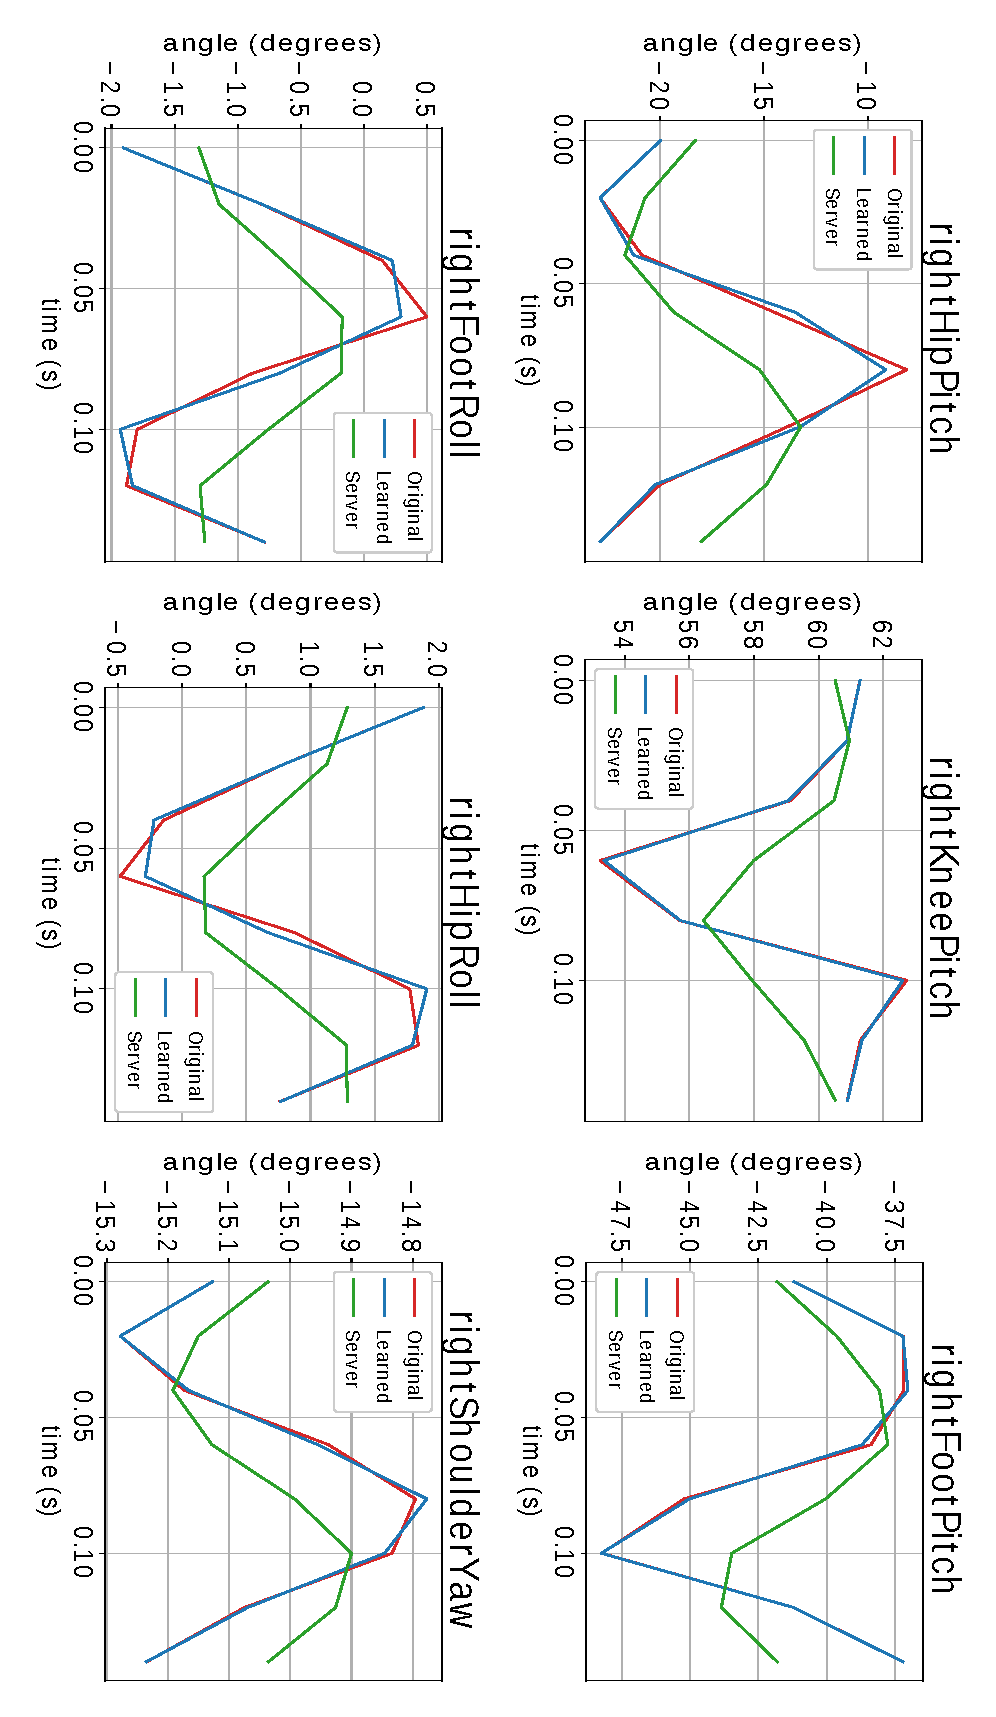
\includegraphics[angle=90,width=1\textwidth]{Cap6/walk_joints_curves}
	\caption{Joints positions, during a period of the walking motion for the original walk, and the learned walk and the joints positions effectively attained, during the learned walking motion.}
	\label{fig:walk_joints_curves}
\end{figure*}

The learned motion has fitted the dataset very well. However, these values were just desired joints. In fact, these values were used as references to joint controllers and were also attenuated due to joint dynamics. Furthermore, this motion was operated in a open-loop fashion, so the agent was not able to correct its own trajectory, and this walks got biased within the simple task of walking straight forward.

Despite the facts previously described, the motion has worked well in a non-competitive scenario\footnote{\label{footnote_walk} Walk results video: https://youtu.be/-pHxTrxllyY}, which was shown in the metrics collected from the Forward Walk test scenario -- agent walking forward from the goal post until the center line of the field -- in Table \ref{tab_walk} and the visual representation in Figure \ref{fig:walkings}.

\begin{table}[htbp]
	\caption{Walk Comparison - Forward Walk}
	\begin{center}
		\begin{tabular}{|c|c|c|c|c|}
			\hline
			\textbf{Walk}&\multicolumn{4}{|c|}{\textbf{Statistics}} \\
			\cline{2-5} 
			\textbf{Type} &\multicolumn{2}{|c|}
			{\textbf{Velocity \((m/s)\)}}
			&\multicolumn{2}{|c|}{\textbf{Y Error \( (m) \) }} \\ 
			\hline
			&
			\textbf{\textit{Mean}} &
			\textbf{\textit{Std}} & \textbf{\textit{Mean}} & \textbf{\textit{Std}} \\
			\hline
			Original Walk & 0.87 & 0.01 & - & -  \\
			\hline
			Learned Walk & 0.23 & 0.01 & 0.96 & 2.63 \\
			\hline
		\end{tabular}
		\label{tab_walk}
	\end{center}
\end{table}


\begin{figure}[!htbp]
	\centering
	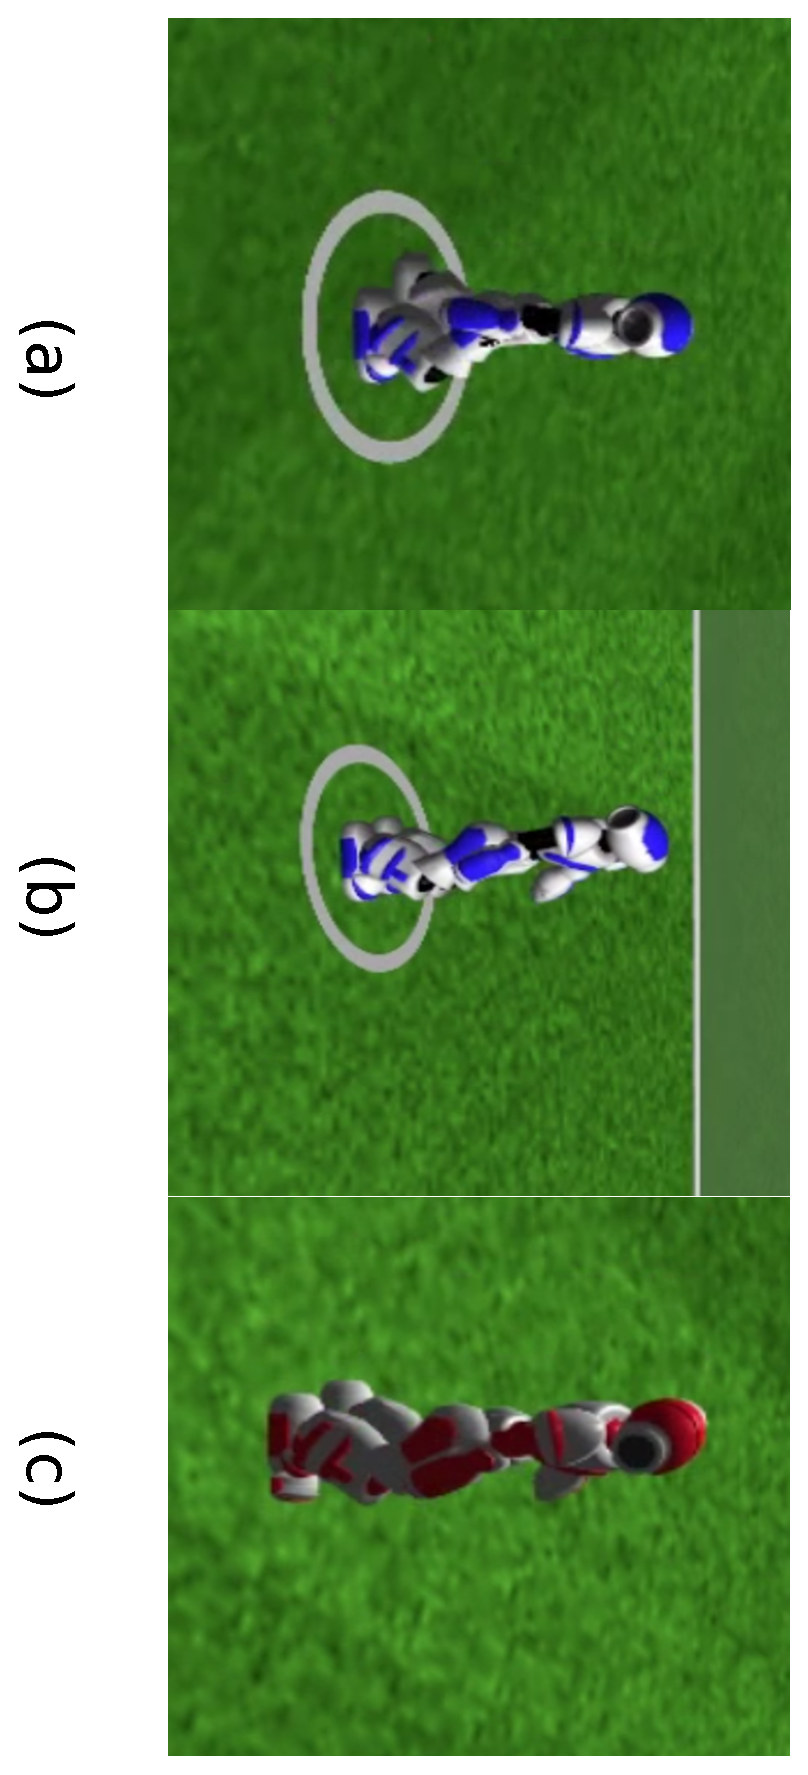
\includegraphics[angle=90, width=1\textwidth]{Cap6/walkings}
	\caption{The walking motions comparison. Figure (a) shows our agent in its regular walk, Figure (b) shows the same agent mimicking UT Austin Villa walk, and Figure (c) shows the UT Austin Villa agent itself performing his own walking motion.}
	\label{fig:walkings}
\end{figure}

\subsubsection{Other motions}

This same framework was used to learn other keyframe motions originated from our agent itself, such as the get up motion. As the cases previously described, the resultant neural network was capable of mimicking the keyframe, by including its interpolation. Hence, all of our keyframe motions could be replaced by neural motions with similar performance.

However, the huge improvement of this method was about mimicking other teams motions. In the Soccer 3D environment, movements like kick and walking have giant impact in team's performance. With this learning framework, our agent was able to mimic multiples movements from several teams.

As an example, we have collected data from UT Austin Villa kick, which was originally optimized by using Deep Reinforcement Learning techniques \cite{mcalpine2017}. Our agent has learned this kick without any additional optimization strategy: we just have used samples collected from the modified server.


\subsection{HLM+RNR}\label{sec:hlmrnr}

In this model, we used the supervised learning model obtained and optimized it towards the task of kicking the ball using RL. The idea is to fine-tune the imitated motion to outperform the performance of original one.

Figure \ref{fig:hlmrewardcurve} shows the reward curve for HLM+RNR model. We can see that the reward double during the course of training.

 \begin{figure}[!htbp]
	\centering
	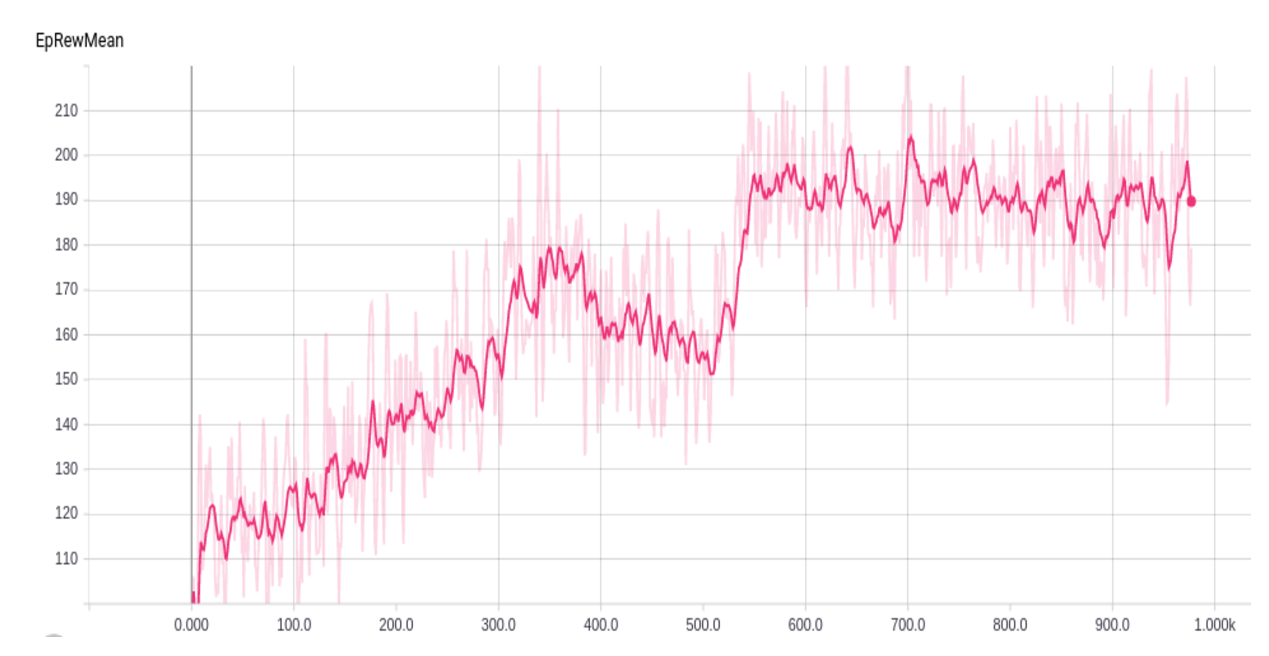
\includegraphics[ width=1\textwidth]{Cap6/hlmreward}
	\caption{HLM+RNR reward curve.}
	\label{fig:hlmrewardcurve}
\end{figure}

Figure \ref{fig:hlmrnrmotionsequence} shows the motion sequence for HLM+RNR model. We see that this motion is very similar to those ones represented in Figure \ref{fig:motions}, even the performance being so different.

The only problem of this training is the integration with the kick behavior of the agent. Here, we optimize just the kick motion. However, the behavior also includes walk to the ball and stops in the right place with the right initial joint values (what we call ball approaching). Then, the performance in the optimization environment is a bit different from actual game situation.


 \begin{figure}[!htbp]
	\centering
	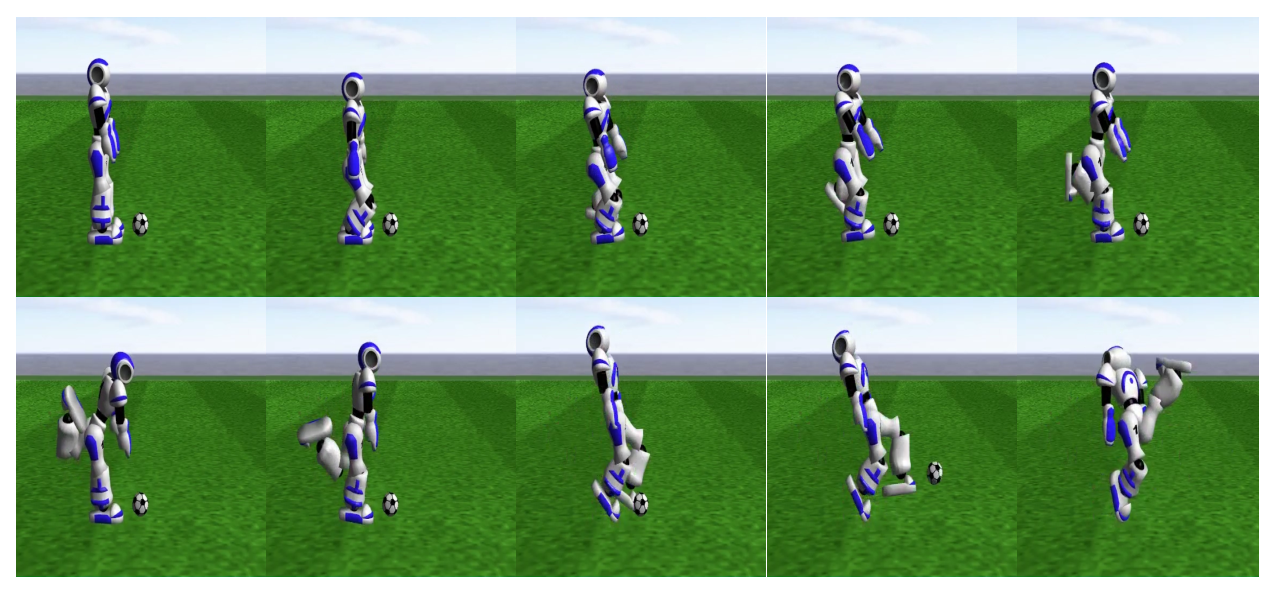
\includegraphics[ width=1\textwidth]{Cap6/hlmmotionsequence}
	\caption{Motion sequence of HLM+RNR model.}
	\label{fig:hlmrnrmotionsequence}
\end{figure}

\subsection{Final Model: HLM+RNR+RET}\label{sec:hlmrnrret}
As final model to explore, we addressed HLM+RNR with Early Termination technique. As described earlier in this work, without it, we collect data that potentially harm training.

In this case, Early Termination consists in end up the episode in two scenarios:

\begin{itemize}
	\item When the robot falls and, therefore, it cannot recover itself; and
	\item When robots kicks the ball, all actions after it will not affect the reward; it is a way to make this reward ``less delayed".
\end{itemize}

In terms of RL training, we did two sessions. In the first one, we parameterized RNR in a way to mainly improve the velocity in frontal direction. The parameters can be found in Appendix \ref{ap:hyperparameters}. Figure \ref{fig:hlmretsess1} shows the reward curve. It results in a kick that optimizes the main problem from the original kick: accuracy. As you can see in Table \ref{tab_kicks_statistics}, the keyframe kick has low accuracy and the learned one is worse, due to the intrinsic error from the learning process. At the end of this first session of RL training, the agent is able to improve its accuracy, although the mean distance being low. Numeric results will be described in next subsection.
 
 
 
 \begin{figure}[!htbp]
 	\centering
 	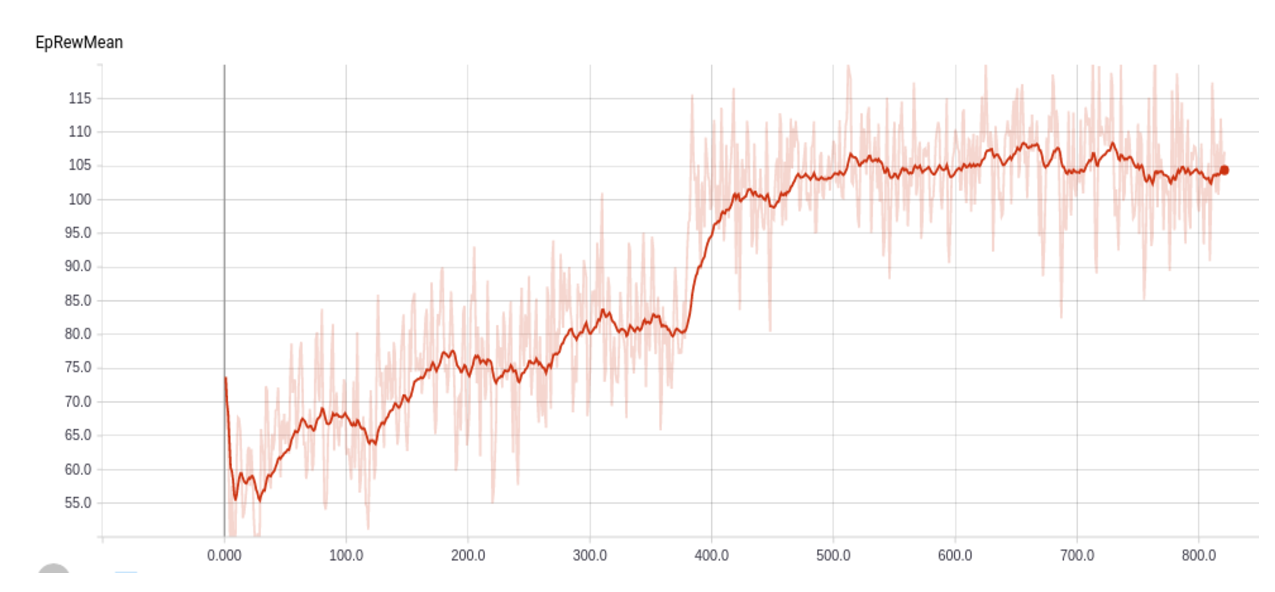
\includegraphics[ width=1\textwidth]{Cap6/hlmretsess1.eps}
 	\caption{The reward curve from the first session of HLM+RNR+RET model.}
 	\label{fig:hlmretsess1}
 \end{figure}

Figure \ref{fig:hlmretsess1motseq} shows the motion sequence after this first session. Although the agent kicks the ball, there is no gain in height. This is a problem for two reasons: first, in a game situation, the ball probably will hits an opponent; second, there is friction between the ball and the ground, decreasing the final reach of it.

 

\begin{figure}[!htbp]
	\centering
	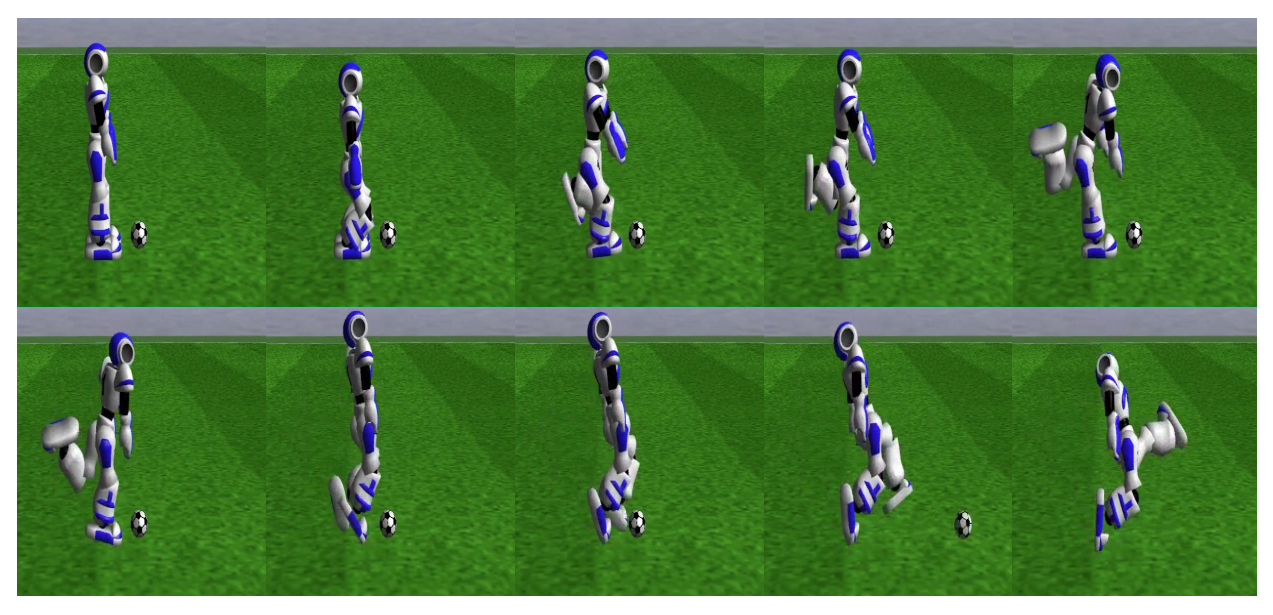
\includegraphics[ width=1\textwidth]{Cap6/hlmretsess1motseq.eps}
	\caption{HLM+RNR+RET motion sequence after first session of training.}
	\label{fig:hlmretsess1motseq}
\end{figure}
 
 In the second session, on the other side, we gave preference to kicks with height, positively reinforcing z-axis velocity. Figures \ref{fig:hlmretsess2} and \ref{fig:hlmretsess2motseq} shows the reward curve and motion sequence, respectively. Even not being so different from motion the sequence of Figure \ref{fig:hlmretsess1motseq}, this training made the agent hits the ball in a way that it gains height, as shown if Figure \ref{fig:hlmretsess2motseq}, resulting in a better general performance than the original keyframe kick.
 
  
 \begin{figure}[!htbp]
 	\centering
 	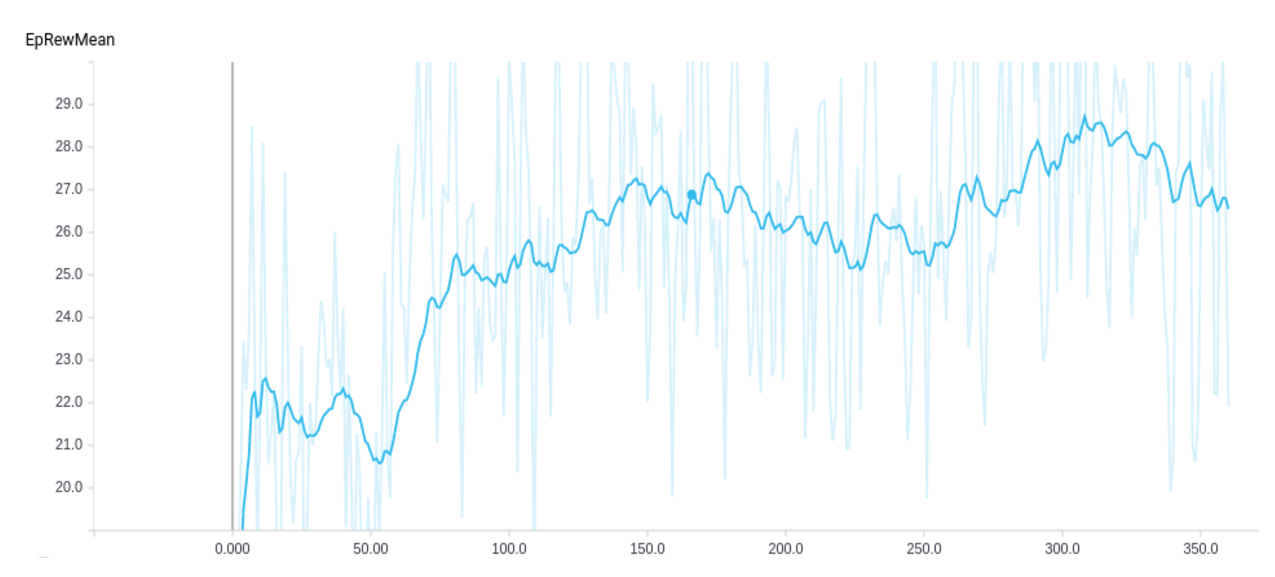
\includegraphics[ width=1.0\textwidth]{Cap6/hlmretsess2}
 	\caption{The reward curve from the second session of HLM+RNR+RET model.}
 	\label{fig:hlmretsess2}
 \end{figure}
 
 \begin{figure}[!htbp]
 	\centering
 	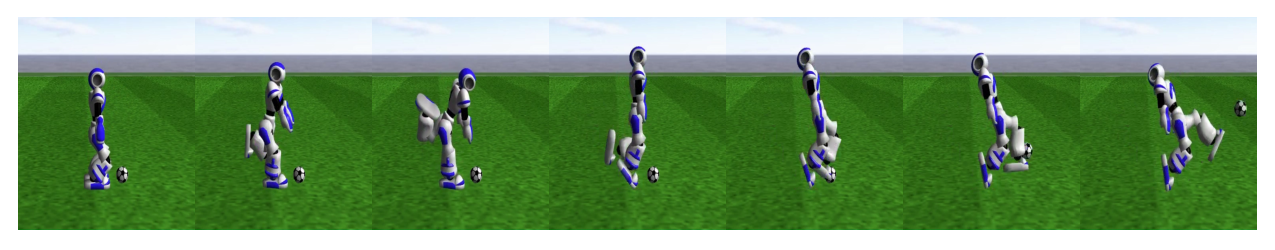
\includegraphics[width=1.0 \textwidth]{Cap6/hlmretsess2motseq}
 	\caption{HLM+RNR+RET motion sequence after second training session.}
 	\label{fig:hlmretsess2motseq}
 \end{figure}

\subsection{Kick Behavior: Numerical Results}\label{sec:kicknumresults}

We created a last test scenario, similar to that from Table \ref{tab_kicks_statistics}, where the agent started 2 meters from the ball, approaches to it and finally kick the ball. This process is conducted by the Kick Behavior, a high-level agent behavior that integrates the walk and kick motions. The idea behind this is to try to simulate better in-game situation and check if the model obtained by these optimizations generalizes well to high-level behaviors, given that we did not optimize any parameter regarding to ball approaching or waking motion.

We collected the distance traveled by ball in axis $x$ and $y$, and the maximum height achieved by the ball during its travel. We also defined a concept of accuracy, considering a ``wrong" kick when the ball does not achieve at least 0.5 meters per second. We ran a hundred of samples and calculated accuracy and mean and standard deviation from other features.

In Table \ref{tab:finaltest}, we compare four different kicks:

\begin{itemize}
	\item \textbf{Original Kick}: the keyframe kick used as reference motion;
	\item \textbf{Learned Kick}: the neural network we learned by supervised learning and using as dataset the Original Kick;
	\item \textbf{HLM+RNR Kick}: the Hybrid Learning Model proposed in Subsection \ref{sec:hlmrnr}; and
	\item \textbf{HLM+RNR+RET Kick}: the Hybrid Learning Model proposed in Subsection \ref{sec:hlmrnrret}.
\end{itemize}

\begin{table}[!htbp]
	\caption{Kick Comparison - General Evaluation}
	\begin{center} 
		\begin{tabular}{|c|c|c|c|c|c|}
			\hline
			\textbf{Kick}&\multicolumn{5}{|c|}{\textbf{Statistics}} \\
			\cline{2-6} 
			\textbf{Type} & \textbf{\textit{Accuracy (\%)}}& \multicolumn{2}{|c|}{\textbf{Distance X(\(m\))}}& 
			\multicolumn{2}{|c|}{\textbf{Distance Z (\(m\))}}\\
			\cline {3-6} 
			& & \textbf{\textit{Mean}}& \textbf{\textit{Std}}
			& \textbf{\textit{Mean}}& \textbf{\textit{Std}}\\
			\hline
			Original Kick & 69.0 & 6.27 & 5.03 & 0.16 & 0.41 \\
			\hline
			Learned Kick & 63.0 & 3.06 & 4.22 & 0.09 & 0.17 \\
			\hline
			HLM+RNR Kick  & 92.0 & 6.52 & 3.89 & 0.33 & 0.55  \\
			\hline
			\textbf{HLM+RNR+RET Kick}  & \textbf{92.0} & \textbf{7.60} & \textbf{3.71} & \textbf{0.45} & \textbf{0.49}  \\
			\hline
		\end{tabular}
		\label{table:finaltest}
	\end{center}
\end{table}

First, we can see that the usage of Early Termination improved the performance results in this test scenario, even the motion being very similar.

As Table \ref{table:finaltest} shows, Hybrid Learning Models outperform both original and learned ones, in this test scenario. General Evaluation means considering the distance traveled by all kicks, even the ones considered ``wrong".

However, it worth mentioning the Effective Evaluation: consider the distance just from ``successful" kicks. We show this evaluation in Table \ref{tab:finaltesteff}.

\begin{table}[!htbp]
	\caption{Kick Comparison - Effective Evaluation}
	\begin{center} 
		\begin{tabular}{|c|c|c|c|c|}
			\hline
			\textbf{Kick}&\multicolumn{4}{|c|}{\textbf{Statistics}} \\
			\cline{2-5} 
			\textbf{Type} &  \multicolumn{2}{|c|}{\textbf{Distance X(\(m\))}}& 
			\multicolumn{2}{|c|}{\textbf{Distance Z (\(m\))}}\\
			\cline {2-5} 
			& \textbf{\textit{Mean}}& \textbf{\textit{Std}}
			& \textbf{\textit{Mean}}& \textbf{\textit{Std}} \\
			\hline
			Original Kick  & \textbf{9.05} & \textbf{3.44} & 0.21 & 0.49 \\
			\hline
			Learned Kick  & 4.82 & 4.46 & 0.12 & 0.21 \\
			\hline
			HLM+RNR Kick & 7.07 & 3.55 & 0.36 & 0.57  \\
			\hline
			\textbf{HLM+RNR+RET Kick} & \textbf{8.26} & \textbf{3.09} & \textbf{0.48} & \textbf{0.49}  \\
			\hline
		\end{tabular}
		\label{tab:finaltesteff}
	\end{center}
\end{table}

We can see from Table \ref{tab:finaltesteff} that when considering just successful kicks, the performance from Original Kick is slightly better. This can be explained by \textbf{performance-stability tradeoff}: the better the performance is, the worse stability should become. Therefore, the training sacrifices performance to gain accuracy -- which we hypothesize that should be better in terms of competition as well.

As final experiment, we applied the HLM+RNR+RET model to a different kind of robot, the Nao with Toe. This one differs from the standard Nao used in the rest of the experiments by having an additional joint in the foot, making it larger. When using the keyframe motion, the Nao with Toe was not able to even kick the ball - very often it kicks the ground because of its large foot.


\begin{table}[!htbp]
	\caption{Kick Evaluation - Nao with Toe}
	\begin{center} 
		\begin{tabular}{|c|c|c|c|c|c|}
			\hline
			\textbf{Kick}&\multicolumn{5}{|c|}{\textbf{Statistics}} \\
			\cline{2-6} 
			\textbf{Type} & \textbf{\textit{Accuracy (\%)}}& \multicolumn{2}{|c|}{\textbf{Distance X(\(m\))}}& 
			\multicolumn{2}{|c|}{\textbf{Distance Z (\(m\))}}\\
			\cline {3-6} 
			& & \textbf{\textit{Mean}}& \textbf{\textit{Std}}
			& \textbf{\textit{Mean}}& \textbf{\textit{Std}}\\
			\hline
			\textbf{Nao with Toe Kick} & \textbf{95.0} & \textbf {9.47} & \textbf{3.43} & \textbf{0.66} & \textbf{0.63} \\ 
			\hline
		\end{tabular}
		\label{tab:naotoe}
	\end{center}
\end{table}

We then applied the framework proposed in this work, which resulted in the values presented in table \ref{tab:naotoe}. It effectively shows the strength of this framework. The RL algorithm, by exploration, was able to adjust the initial motion to this kind of robot, resulting in a even better motion than the original keyframe based on standard Nao. 